\documentclass[12pt]{article}
\usepackage[english]{babel}
\usepackage[utf8]{inputenc}
\usepackage{amsmath, amssymb, amsthm}
\usepackage{graphicx}
\usepackage{hyperref}
\usepackage[margin=.75in]{geometry}
\usepackage{xcolor}
\usepackage{tikz}

\newcommand{\id}{\text{id}}
\newcommand{\od}{\text{od}}

\setlength{\topmargin}{0pt}
\setlength{\headsep}{0pt}
\textheight = 600pt

\title{Graph Theory \\ Homework 12}
\author{Ben Kallus and Ryan Friedman}
\date{Due Thursday, April 8}

\begin{document}
\maketitle

\medskip\noindent\textbf{8.18} Proposition: There exists a 5-regular graph with no 1-factor.
\begin{proof}
    The graph shown below is clearly 5-regular, but removing the vertex on top would create 5 odd components, so this graph does not satisfy the odd component condition, and therefore has no 1-factor.
    \begin{center}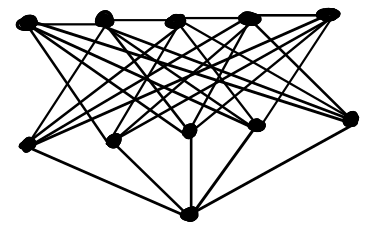
\includegraphics[scale=.4]{pic1.png}\end{center}
\end{proof}

\newpage\noindent\textbf{8.20} Proposition: Every 3-regular graph with at most two bridges contains a 1-factor.
\begin{proof}
    Let $G$ be a 3-regular graph, and let $\emptyset \neq S \subseteq V(G)$.
    Let $G_1, \hdots, G_\ell$ denote the odd components of $G-S$, and let $G_{\ell+1}, \hdots, G_j$ denote the even components of $G-S$.
    Then, $$V(G) = S \sqcup G_1 \sqcup \hdots \sqcup G_{\ell} \sqcup G_{\ell+1} \hdots \sqcup G_j.$$
    Since $G_1, \hdots, G_{\ell}$ are even components, the parity of $|V(G)|$ is equal to the parity of $|S \sqcup G_{\ell+1} \sqcup \hdots \sqcup G_j|$.
    Because $G$ is 3-regular, it must have an even number of vertices by the Handshaking Lemma.
    Thus, $|S \sqcup G_{\ell+1} \sqcup \hdots \sqcup G_j|$ is even, so the parity of $|S|$ is equal to the parity of $|G_{\ell+1} \sqcup \hdots \sqcup G_j|$.
    Since each of $G_\ell, \hdots, G_j$ is odd, it must be that $|S|$ has the same parity as $k_o(G - S)$.

    We now show that $k_o(G - S)$ is at most $|S|$.
    Since this is clearly true if $k_o(G - S) = 0$, we consider the case in which $k_o(G-S) = \ell \geq 1$.
    Then, $G-S$ has odd components $G_1, \hdots, G_{\ell}$.
    Let $X_i$ $(1 \leq i \leq \ell)$ denote the set of edges with one endvertex in $S$ and the other in $G_i$.
    Since every vertex of $G_i$ has degree 3 in $G$ and the sum of the degrees of the vertices in the graph $G_i$ is even, $|X_i|$ is odd.
    Because $G$ has at most 2 bridges, there are at most 2 values of $i$ such that $|X_i| = 1$, and at least $\ell - 2$ values of $i$ such that $|X_i| \geq 3$.
    Thus, there are at most $3(\ell - 2) + 2$ edges joining the vertices of $S$ and the vertices of $G-S$.
    Note that because $G$ is 3-regular, there at most $3|S|$ edges joining vertices in $S$ and vertices in $G-S$.
    Thus, $$3(\ell - 2) + 2 \leq 3|S|.$$
    Therefore, $$3\left(\ell - \frac43\right) \leq 3|S|.$$
    Then, $$\ell - \frac43 \leq |S|.$$
    Since $\ell$ and $|S|$ have the same parity, then if $\ell > |S|$, $\ell - 2 \geq |S|$.
    In that case, $\ell - \frac43 \not\leq |S|$, so it must be that $\ell \leq |S|$.
    Thus, $k_o(G-S) \leq |S|$.
\end{proof}

\newpage\noindent\textbf{8.24} Proposition: Every 3-regular bridgeless graph contains a 2-factor.
\begin{proof}
    Let $G$ be a 3-regular bridgeless graph.
    By Theorem 8.11, $G$ contains a 1-factor $F_1$.
    Since $G$ is 3-regular, $G-F_1$ is 2-regular.
    Since $G$ is 3-regular and $F_1$ is a 1-factor, $G-F_1$ is a spanning subgraph of $G$.
    Thus, $G-F_1$ is a 2-factor for $G$.
\end{proof}

\newpage\noindent\textbf{8.26} For any 2-factorization of $G$, exactly one of the 2-factors is a Hamiltonian cycle of $G$.
\begin{proof}
    Let $F_1, F_2$ be a 2-factorization of $G$.
    Suppose without loss of generality that $F_1$ contains exactly one of the edges $u_1v_1, u_5v_5$.
    Then, that edge would be a bridge in $F_1$, because the only edges connecting the top and bottom portions of $G$ are $u_1v_1$ and $u_5v_5$.
    Thus, $F_1$ cannot consist only of cycles, so it must not be 2-regular, and is therefore not a 2-factor of $G$.
    Thus, $F_1$ either contains both $u_1v_1$ and $u_5v_5$, or it contains neither.
    If $F_1$ contains neither of these edges, then $F_2$ must contain both of them, so we assume without loss of generality that $F_1$ contains both $u_1v_1$ and $u_5v_5$.
    Since $G-u_1v_1 - u_5v_5$ is disconnected, $F_2$ must not be a Hamiltonian cycle.
    Since $F_1$ includes $u_1v_1$ and $u_5v_5$, $F_1$ contains a cycle $C = (u_5,v_5, \hdots, v_1, u_1, \hdots v_5)$.
    Observe that all $v_5-v_1$ paths in $G$ that do not include $v_5u_5$ either have length 2 or length 4.
    If $C$ contains a length 2 path between $v_5$ and $v_1$, then $C$ does not visit two vertices in the lower portion of $G$, so one of $F_1$'s components is isomorphic to $K_2$.
    Then, $F_1$ would not be 2-regular.
    Thus, $C$ must contain a length 4 path between $v_5$ and $v_1$ that does not include $v_5u_5$, so all vertices in the bottom portion of $G$ must be present in $C$.
    By a symmetric argument, all vertices in the top portion of $G$ must be present in $C$, so $C = F_1$ is a Hamiltonian cycle.
\end{proof}


\newpage\noindent\textbf{8.28} If a 6-regular graph $G$ contains two edge-disjoint 1-factors, then it is 3-factorable.
\begin{proof}
    Let $G$ be a 6-regular graph with two edge-disjoint 1-factors $F_1, F_2$.
    Then, $G - F_1 - F_2$ is a 4-regular spanning subgraph of $G$.
    Then, by Theorem 8.16, $G-F_1 -F_2$ is 2-factorable into $F_3, F_4$.
    Consider $F_1 \cup F_3$ and $F_2 \cup F_4$.
    Since each of the $F_i$s is edge-disjoint, $F_1 \cup F_3$ and $F_2 \cup F_4$ are therefore 3-regular.
    Since $F_1$ and $F_2$ are spanning subgraphs of $G$, $F_1 \cup F_3$ and $F_2 \cup F_4$ must also be spanning subgraphs of $G$.
    Thus, $G$ is 3-factorable into $F_1 \cup F_3, F_2 \cup F_4$.
\end{proof}


\end{document}
